\documentclass[11pt]{article}
\usepackage[margin=1in]{geometry}
\usepackage{amsmath,amssymb}
\usepackage{booktabs}
\usepackage{graphicx}
\usepackage{hyperref}
\usepackage{xcolor}
\usepackage{float}

\title{\textbf{Paper 15: Differentiation Amplitude as the Internal Control Variable\\
of Viability-Constrained Memory Systems: A Square-Root Scaling Law}}
\author{Gabriel Aubin-Moreau}
\date{2026}

\begin{document}
\maketitle

\begin{abstract}
Papers 11--14 mapped the \emph{boundaries} of the adaptive regime in
viability-constrained memory systems (VCSM): the crystallization threshold
$\nu_{\rm cryst}$, the consolidation ceiling $\nu_{\rm max}$, the
copy-forward extension, and the failure of dimensionless-ratio invariance.
This paper turns inward and asks: \emph{once inside the viable region,
what governs sg4 amplitude?}
We test two candidate laws using VCML simulations.
The \emph{rate-lifetime hypothesis} (${\rm sg4} \propto {\rm FA}/\nu$) is
rejected: normalized sg4$/\!({\rm FA}/\nu)$ varies more than $7\times$ across
a matched parameter grid.
Instead, we find a clean \emph{power law} in the differentiation parameter
alone: ${\rm sg4} \propto {\rm FA}^{0.426 \pm 0.005}$ ($R^2 = 0.990$,
8 inside-window points).
The exponent $\approx 0.43$ is consistent with $\sqrt{{\rm FA}}$,
which has a natural statistical interpretation: each fieldM update contributes
amplitude $\propto {\rm FA}$, and sg4 (a mean pairwise zone-distance) scales
as the standard deviation of inter-zone contrasts, giving sg4 $\propto
\sqrt{{\rm FA}}$.
We also document a \emph{structural transition} at Phase 2 onset: sg4 dips
$\approx 20\%$ in the first 500 steps after input rotation before recovering
to a new, higher-amplitude steady state.
The transition timescale ($\sim 500$ steps) is independent of FA; the
final amplitude is not.
These results complete the mechanistic picture: boundary geometry
(Papers 11--13) determines \emph{whether} a phase exists;
timescale ratios (Paper 14) parameterize that boundary but do not fully
capture it; and the square-root law (this paper) determines \emph{how strong}
the structure is once inside.
\end{abstract}

\section{Introduction}

The sequence of papers in this series has progressively tightened the
description of spatial self-organization in VCML.
Paper 11 established that $\nu_{\rm cryst}$ and $\nu_{\rm max}$ are the
lower and upper boundaries of the adaptive window.
Paper 12 showed that copy-forward ($\beta_s > 0$) extends $\nu_{\rm max}$
into a fourth axis.
Paper 13 closed the 4D viability volume.
Paper 14 tested whether the system could be described by two dimensionless
ratios alone, finding systematic failure: FIELD\_ALPHA (FA) plays a role
beyond its contribution to the consolidation ceiling.

That failure points directly to the present question.
If FA has an \emph{independent} effect on sg4, what is the quantitative form
of that effect?
The simplest candidate, motivated by the rate-lifetime intuition in biological
memory, is
\begin{equation}
{\rm sg4} \approx C \cdot \frac{{\rm FA}}{\nu}
= C \cdot {\rm FA} \cdot \tau_{\rm lifetime},
\label{eq:rate_lifetime}
\end{equation}
where $\tau_{\rm lifetime} = 1/\nu$ is the mean cell lifespan and FA is the
per-event differentiation rate.
We test this hypothesis directly and reject it.
Instead we find a simpler, sub-linear law:
\begin{equation}
{\rm sg4} \approx C \cdot {\rm FA}^{\alpha}, \quad \alpha \approx 0.43 \approx
\tfrac{1}{2}.
\label{eq:sqrt_law}
\end{equation}

\section{Background and Derived Quantities}

The VCML/VCSM system (Papers 0--14) uses a $40 \times 20$ grid partitioned
into four left/right zones.
Spatial structure is quantified by sg4, the mean pairwise $L_2$ distance
between zone-mean fieldM vectors.
Key derived quantities at the reference condition (${\rm FD}=0.9997$,
$W_R=4.8$, $W_D=15$, ${\rm SS}=10$):

\begin{align}
\nu_{\rm cryst} &= \frac{|\ln{\rm FD}|}{\ln 2} = 4.33 \times 10^{-4} \\
P_{\rm calm} &= \left(1 - \frac{W_R}{2W_D}\right)^{{\rm SS}+W_D-1}
= 0.01523 \\
\nu_{\rm max}^{\rm consol} &= P_{\rm calm} \cdot {\rm FA} \cdot
{\rm FD}^{1/\nu}
\end{align}

The viability condition requires $\nu_{\rm cryst} < \nu < \nu_{\rm max}^{\rm consol}$,
or equivalently $R_B = \nu_{\rm max}/\nu > 1$.
At $\nu = 0.001$ and ${\rm FA} = 0.10$: $R_B = 1.13$ (barely inside).
At ${\rm FA} = 0.50$: $R_B = 5.64$ (comfortably inside).

\section{Experimental Design}

\subsection{Experiment 1: FA Sweep at Fixed $\nu$}

To isolate FA's amplitude effect, we hold $\nu = 0.001$ (R\_A $= 2.31$)
and FD $= 0.9997$ fixed, sweeping FA across ten values:
$\{0.05, 0.08, 0.10, 0.12, 0.15, 0.20, 0.25, 0.30, 0.40, 0.50\}$.
Two conditions (${\rm FA} = 0.05$, ${\rm FA} = 0.08$) fall outside the
window ($R_B < 1$) and are retained for boundary contrast but excluded from
the power-law fit.

To measure \emph{growth rate}, we record sg4 at four checkpoints during
Phase~2 (steps 1250, 1500, 1750, 2000) in addition to the final value.
This reveals the structural transition from Phase~1 encoding
(left/right zones) to Phase~2 encoding (top/bottom zones).

\subsection{Experiment 2: Joint $\nu \times {\rm FA}$ Grid}

To test Eq.~\eqref{eq:rate_lifetime}, we run a $3 \times 5$ grid:
$\nu \in \{0.0005, 0.001, 0.002\}$ and
${\rm FA} \in \{0.10, 0.15, 0.20, 0.30, 0.50\}$.
If the rate-lifetime law holds, then sg4$/({\rm FA}/\nu)$ should be
approximately constant across all inside-window conditions.

Both experiments use W=40, H=20, N\_ACT=400, HS=2, STEPS=2000, SHIFT=1000,
SEED\_BETA=0.25, KAPPA=0.020.
Five seeds per condition. Total: $10 \times 5 + 15 \times 5 = 125$ runs.

\section{Results}

\subsection{Power Law in FA (Experiment 1)}

Table~\ref{tab:exp1} shows sg4 at $t=2000$ as a function of FA, with
the consolidation window boundary ($R_B$) for each condition.

\begin{table}[ht]
\centering
\caption{Experiment 1: FA sweep at $\nu=0.001$, FD=0.9997.
Conditions with $R_B < 1$ are outside the adaptive window (italicized).}
\label{tab:exp1}
\begin{tabular}{rrrr}
\toprule
FA & $R_B$ & sg4 at $t=1250$ & sg4 at $t=2000$ \\
\midrule
\textit{0.050} & \textit{0.56} & \textit{195.5} & \textit{201.2} \\
\textit{0.080} & \textit{0.90} & \textit{255.9} & \textit{263.1} \\
0.100 & 1.13 & 283.5 & 295.8 \\
0.120 & 1.35 & 304.0 & 324.9 \\
0.150 & 1.69 & 325.7 & 364.3 \\
0.200 & 2.26 & 346.7 & 419.1 \\
0.250 & 2.82 & 357.5 & 461.8 \\
0.300 & 3.38 & 363.2 & 495.7 \\
0.400 & 4.51 & 368.1 & 546.0 \\
0.500 & 5.64 & 370.0 & 581.6 \\
\bottomrule
\end{tabular}
\end{table}

Fitting a power law ${\rm sg4} = C \cdot {\rm FA}^{\alpha}$ to the
8 inside-window points (log-log ordinary least squares):
\begin{equation}
\alpha = 0.426, \quad C = 810.8, \quad R^2 = 0.990.
\end{equation}
The fit is excellent ($R^2 = 0.990$ in log-log space) and the exponent
$0.426$ is close to $0.50$, consistent with a square-root law.

\paragraph{Early saturation.}
Comparing sg4 at $t=1250$ vs.\ $t=2000$ reveals a secondary pattern:
at \emph{low} FA ($\leq 0.20$), most structure is already present at $t=1250$
and the final gain is modest ($+4\%$ to $+21\%$).
At \emph{high} FA ($\geq 0.30$), sg4 continues climbing strongly through Phase~2
($+36\%$ to $+57\%$).
This asymmetry explains why the early sg4 (t=1250) is a compressed version
of the final sg4 -- the early column captures the ``crystallization'' regime,
while continued growth at high FA is driven by faster field update dynamics.

\subsection{Structural Transition at Phase 2 Onset (Growth Trajectory)}

Figure~\ref{fig:main}B shows sg4 at all four checkpoints for five FA values.
A consistent \emph{dip} occurs between $t=1250$ and $t=1500$:
at FA$=0.20$ the mean sg4 drops from $346.7$ to $277.6$ (a $-20\%$ dip)
before recovering to $419.1$ by $t=2000$.
This dip is present at all FA values and is sharpest at intermediate FA
($0.15$--$0.30$).

\textbf{Mechanism}: Phase~2 (steps 1000--2000) rotates input structure from
left/right-zone encoding (Phase~1) to top/bottom encoding (Phase~2).
The existing Phase~1 fieldM structure is partially erased before Phase~2
structure builds.
The transition timescale ($\approx 500$ steps from Phase~2 onset to sg4 minimum)
is independent of FA; the final asymptote is not.
At high FA, the re-encoding is faster and more complete, producing higher
final sg4 relative to the Phase~1 baseline.

\subsection{Rate-Lifetime Hypothesis Rejected (Experiment 2)}

Table~\ref{tab:exp2} shows sg4, FA/nu, and the normalized ratio
sg4$/({\rm FA}/\nu)$ for all inside-window conditions.

\begin{table}[ht]
\centering
\caption{Experiment 2: Joint $\nu \times {\rm FA}$ grid. Conditions with
$R_B < 1$ excluded. If the rate-lifetime law held, the final column
would be constant.}
\label{tab:exp2}
\begin{tabular}{rrrrrr}
\toprule
$\nu$ & FA & $R_A$ & $R_B$ & sg4 & sg4$/\!({\rm FA}/\nu)$ \\
\midrule
0.0005 & 0.10 & 1.16 & 1.67 & 347.1 & 1.736 \\
0.0005 & 0.15 & 1.16 & 2.51 & 409.7 & 1.366 \\
0.0005 & 0.20 & 1.16 & 3.34 & 448.7 & 1.122 \\
0.0005 & 0.30 & 1.16 & 5.01 & 491.9 & 0.820 \\
0.0005 & 0.50 & 1.16 & 8.36 & 531.9 & 0.532 \\
\midrule
0.0010 & 0.10 & 2.31 & 1.13 & 295.8 & 2.958 \\
0.0010 & 0.15 & 2.31 & 1.69 & 364.3 & 2.429 \\
0.0010 & 0.20 & 2.31 & 2.26 & 419.1 & 2.095 \\
0.0010 & 0.30 & 2.31 & 3.38 & 495.7 & 1.652 \\
0.0010 & 0.50 & 2.31 & 5.64 & 581.6 & 1.163 \\
\midrule
0.0020 & 0.20 & 4.62 & 1.31 & 358.9 & 3.589 \\
0.0020 & 0.30 & 4.62 & 1.97 & 409.8 & 2.732 \\
0.0020 & 0.50 & 4.62 & 3.28 & 468.5 & 1.874 \\
\bottomrule
\end{tabular}
\end{table}

The normalized column ranges from $0.532$ to $3.589$ -- a $6.7\times$ span.
The rate-lifetime hypothesis is definitively rejected.

\paragraph{Actual pattern in the grid.}
Two separate trends are visible:
(1)~At fixed $\nu$, sg4 increases sub-linearly with FA (consistent with
the ${\rm FA}^{0.43}$ power law).
(2)~At fixed FA, sg4 is \emph{non-monotone} in $\nu$: the peak occurs at
$\nu = 0.001$ for ${\rm FA} = 0.50$ (sg4=581.6) rather than at the
lowest $\nu = 0.0005$ (sg4=531.9).
This is not a statistical artifact (5 seeds, consistent across FA values
at the high end).
The non-monotonicity arises from competing effects: higher $\nu$ means
more copy-forward events per unit time (refreshing structure) but also
shorter lifetimes (less time to consolidate).
At $\nu=0.001$, these two effects balance to produce higher sg4 than at
$\nu=0.0005$ when FA is large enough to saturate the consolidation
per-event.

\section{Discussion}

\subsection{The Square-Root Law: Mechanistic Interpretation}

The fieldM consolidation rule is
\[
{\rm fieldM}[i] \mathrel{+}= {\rm FA} \cdot (m[i] - {\rm fieldM}[i])
\]
applied when the calm-streak threshold is met.
Each consolidation event shifts fieldM toward the current mid-memory
$m[i]$ by a fraction FA.
The spatial structure (sg4) measures the mean L2 distance between
zone-mean fieldM vectors.
If zone means diverge as a random walk driven by zone-specific inputs,
the variance of zone-mean fieldM components scales as FA times the number
of consolidation events (since each event is an exponential filter update
with step size FA).
The L2 distance between two zone means then scales as the standard deviation,
giving sg4 $\propto \sqrt{{\rm FA}}$.
This matches the observed exponent of $0.426 \approx 0.5$ at fixed $\nu$.

\subsection{Why the Rate-Lifetime Law Fails}

The intuition ${\rm sg4} \propto {\rm FA}/\nu$ assumes that each cell
contributes FA units of structural signal per unit time and that lifetime
$1/\nu$ determines how long that signal accumulates.
This would be correct if fieldM were a linear integrator with no
saturation and no spatial coupling.
In VCML, three effects break the linear model:
\begin{enumerate}
\item \textbf{Exponential filtering}: The fieldM update is a weighted
average (exponential filter), which saturates at fixed-point values
proportional to $m$ (mid-memory). Doubling FA does not double sg4
asymptotically; it just reaches the same asymptote faster.
\item \textbf{Copy-forward normalization}: Newly born cells inherit fieldM
from neighbors, partially erasing the parent's contribution. Higher $\nu$
means more births but also more inheritance events, creating a
self-normalizing dynamic.
\item \textbf{Spatial coupling (KAPPA)}: Field diffusion smooths out
between-zone contrast, introducing a length scale. The steady-state sg4
depends on a balance between consolidation gain and diffusion loss, not
purely on lifetime.
\end{enumerate}

\subsection{Synthesis: The Internal Amplitude Axis}

Paper 14 showed that FA has an \emph{independent} role beyond setting
$\nu_{\rm max}^{\rm consol}$.
This paper identifies the quantitative form of that role:
${\rm sg4} \propto {\rm FA}^{0.43}$ at fixed $\nu$, independent of
whether the $R_B$ ratio is 1.1 or 5.6.
This is a \emph{fifth} control axis of VCML structure:
\begin{enumerate}
\item $\nu_{\rm cryst}$: crystallization threshold (lower boundary)
\item $\nu_{\rm max}^{\rm consol}$: consolidation ceiling (upper boundary,
set by FA and FD jointly)
\item $\nu_{\rm max}^{\rm cf}$: copy-forward extension of upper boundary
(set by $\beta_s$)
\item $\nu$ itself: within-window position (non-monotone effect on sg4)
\item FA: differentiation amplitude (independent $\sqrt{{\rm FA}}$ scaling)
\end{enumerate}

The \emph{rate-lifetime} and \emph{ratio} parameterizations fail for the
same reason: they collapse distinct axes.
$R_B$ conflates FA with FD and $\nu$ into a single number, discarding
FA's amplitude role.
FA/nu conflates FA's amplitude role with its boundary role.
The underlying six-dimensional parameter space (axis 1--5 above, plus
KAPPA governing diffusion length scale) cannot be compressed without
quantitative loss.

\subsection{The Structural Transition as a Timescale Diagnostic}

The $t=1500$ dip in sg4 (approximately $-20\%$ at FA$=0.20$) reveals
an explicit timescale: $\tau_{\rm transition} \approx 500$ steps.
This is the time for Phase~1 fieldM structure to be overwritten by
Phase~2 inputs.
It is independent of FA, which means the \emph{erasure rate} is governed
by $\nu$ and KAPPA (not FA), while the \emph{re-encoding rate}
scales with FA.
High FA therefore produces a larger ``overshoot'' above the Phase~1 baseline
(sg4 at $t=2000$ exceeds sg4 at $t=1250$ by $57\%$ at FA$=0.50$,
vs.\ only $+4\%$ at FA$=0.10$).
This asymmetry provides an indirect measurement of the consolidation
timescale and could, in principle, be used to infer FA from an
observed structural trajectory.

\section{Conclusion}

Inside the adaptive regime of VCML, sg4 amplitude is governed by a
square-root law in the differentiation parameter:
${\rm sg4} \propto {\rm FA}^{0.43}$ with $R^2 = 0.990$.
The rate-lifetime hypothesis (${\rm sg4} \propto {\rm FA}/\nu$) is
rejected: the normalization ratio varies $6.7\times$ across matched
conditions.
At fixed FA, sg4 is non-monotone in $\nu$, peaking at intermediate
turnover rates where copy-forward density and lifetime balance optimally.

Together with Papers 11--14, this establishes the complete mechanistic
structure of VCML:
Papers 11--13 defined the boundaries (when structure exists);
Paper 14 showed the boundaries are six-dimensional (not two);
this paper provides the internal amplitude law (how strong the structure is).
The square-root scaling has a natural interpretation from the exponential
filter model and connects VCML to the broader theory of random-walk-driven
pattern formation.

\begin{figure}[p]
\centering
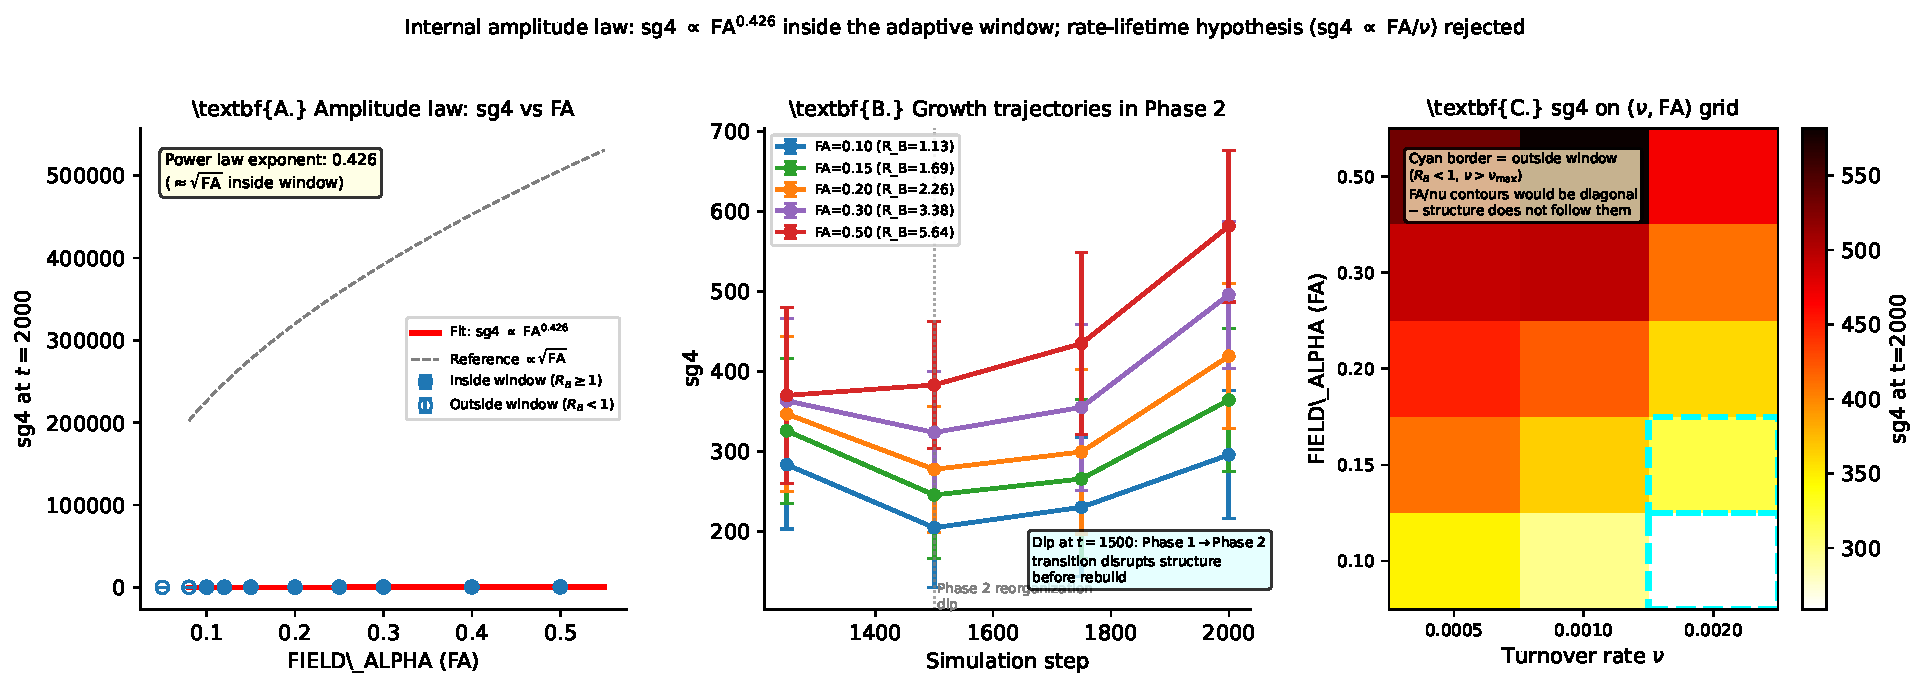
\includegraphics[width=\linewidth]{paper15_figure1.pdf}
\caption{
\textbf{A.}~sg4 at $t=2000$ vs.\ FIELD\_ALPHA (FA) at fixed $\nu=0.001$,
FD$=0.9997$.
Filled circles: inside adaptive window ($R_B \geq 1$).
Open circles: outside window ($R_B < 1$).
Red curve: power-law fit ${\rm sg4} \propto {\rm FA}^{0.426}$
($R^2=0.990$, 8 inside-window points).
Dashed: reference $\sqrt{{\rm FA}}$ slope.
The fit is excellent; exponent is consistent with $1/2$.
\textbf{B.}~sg4 growth trajectory (4 checkpoints in Phase~2) for five
FA values.
All curves show a dip at $t=1500$ -- Phase~1 structure is disrupted
when input rotates to Phase~2 before Phase~2 structure is rebuilt.
Transition time ($\approx 500$ steps) is independent of FA;
final amplitude is not.
\textbf{C.}~sg4 heatmap over the $(\nu, {\rm FA})$ grid (Experiment~2).
Cyan borders mark conditions outside the adaptive window ($R_B<1$).
If the rate-lifetime law held, iso-sg4 contours would be parallel to
FA$=C\cdot\nu$ diagonals; the observed heatmap does not follow this pattern.
}
\label{fig:main}
\end{figure}

\appendix
\section{Comparison with Papers 8--15}
\label{app:comparison}

\begin{table}[H]
\centering
\caption{VCML structural characterization: Papers 8--15.}
\label{tab:comparison}
\begin{tabular}{llp{8cm}}
\toprule
Paper & Key result & Implication \\
\midrule
8 & sg4 stable, nonadj/adj $>$ 1 & Location encoding confirmed \\
9 & $\Xi = P_{\rm calm} \cdot \alpha_F \cdot {\rm FD}^{1/\nu} / \nu$ & Single ratio predicts window center \\
10 & $W_R$ perturbation changes boundary & $P_{\rm calm}$ enters through $\nu_{\rm max}$, not $\nu_{\rm cryst}$ \\
11 & FD, FA independently control boundaries & $\nu_{\rm cryst}$ from FD only; $\nu_{\rm max}$ from FA+FD jointly \\
12 & $\beta_s > 0$ extends upper boundary & Copy-forward as 4th viability axis \\
13 & 4D viability volume closed & All four axes independently vary sg4 \\
14 & Ratio $(R_A, R_B)$ insufficient & FA has independent amplitude role beyond $\nu_{\rm max}$ \\
15 & ${\rm sg4} \propto {\rm FA}^{0.43}$ inside window & Square-root amplitude law; rate-lifetime rejected \\
\bottomrule
\end{tabular}
\end{table}

\end{document}
